%  A simple AAU report template.
%  2015-05-08 v. 1.2.0
%  Copyright 2010-2015 by Jesper Kjær Nielsen <jkn@es.aau.dk>
%
%  This is free software: you can redistribute it and/or modify
%  it under the terms of the GNU General Public License as published by
%  the Free Software Foundation, either version 3 of the License, or
%  (at your option) any later version.
%
%  This is distributed in the hope that it will be useful,
%  but WITHOUT ANY WARRANTY; without even the implied warranty of
%  MERCHANTABILITY or FITNESS FOR A PARTICULAR PURPOSE.  See the

%  GNU General Public License for more details.
%
%  You can find the GNU General Public License at <http://www.gnu.org/licenses/>.
%
%  A simple AAU report template.
%  2015-05-08 v. 1.2.0
%  Copyright 2010-2015 by Jesper Kjær Nielsen <jkn@es.aau.dk>
%
%  This is free software: you can redistribute it and/or modify
%  it under the terms of the GNU General Public License as published by
%  the Free Software Foundation, either version 3 of the License, or
%  (at your option) any later version.
%
%  This is distributed in the hope that it will be useful,
%  but WITHOUT ANY WARRANTY; without even the implied warranty of
%  MERCHANTABILITY or FITNESS FOR A PARTICULAR PURPOSE.  See the
%  GNU General Public License for more details.
%
%  You can find the GNU General Public License at <http://www.gnu.org/licenses/>.
%
\documentclass[11pt,twoside,a4paper,openright]{report}
%%%%%%%%%%%%%%%%%%%%%%%%%%%%%%%%%%%%%%%%%%%%%%%%
% Language, Encoding and Fonts
% http://en.wikibooks.org/wiki/LaTeX/Internationalization
%%%%%%%%%%%%%%%%%%%%%%%%%%%%%%%%%%%%%%%%%%%%%%%%
% Select encoding of your inputs. Depends on
% your operating system and its default input
% encoding. Typically, you should use
%   Linux  : utf8 (most modern Linux distributions)
%            latin1 
%   Windows: ansinew
%            latin1 (works in most cases)
%   Mac    : applemac
% Notice that you can manually change the input
% encoding of your files by selecting "save as"
% an select the desired input encoding. 
\usepackage[utf8]{inputenc}
% Make latex understand and use the typographic
% rules of the language used in the document.
\usepackage[english]{babel}
%\addto\captionsenglish{\renewcommand{\chaptername}{Kapitel}}
%\addto\captionsenglish{\renewcommand{\contentsname}{Indhold}}
%\addto\captionsenglish{\renewcommand{\prefacename}{Titelblad}}
%\addto\captionsenglish{\renewcommand{\figurename}{Figur}}
%\addto\captionsenglish{\renewcommand{\tablename}{Tabel}}
%\addto\captionsenglish{\renewcommand{\appendixname}{Appendiks}}
% Use the palatino font
\usepackage[sc]{mathpazo}
\linespread{1.05}         % Palatino needs more leading (space between lines)
% Choose the font encoding
\usepackage[T1]{fontenc}
\newcommand{\hashsharp}{$^\#$}
%%%%%%%%%%%%%%%%%%%%%%%%%%%%%%%%%%%%%%%%%%%%%%%%
% Graphics and Tables
% http://en.wikibooks.org/wiki/LaTeX/Importing_Graphics
% http://en.wikibooks.org/wiki/LaTeX/Tables
% http://en.wikibooks.org/wiki/LaTeX/Colors
%%%%%%%%%%%%%%%%%%%%%%%%%%%%%%%%%%%%%%%%%%%%%%%%
% load a colour package
\usepackage{xcolor}
\definecolor{aaublue}{RGB}{33,26,82}% dark blue
\definecolor{gray}{RGB}{200,200,200} %light gray
% The standard graphics inclusion package
\usepackage{graphicx}
% Set up how figure and table captions are displayed
\usepackage{caption}
\usepackage{subcaption}
\captionsetup{%
  font=footnotesize,% set font size to footnotesize
  labelfont=bf % bold label (e.g., Figure 3.2) font
}
% Make the standard latex tables look so much better
\usepackage{array,booktabs}
% Enable the use of frames around, e.g., theorems
% The framed package is used in the example environment
\usepackage{framed}
\usepackage{float}
\usepackage{enumitem} % Enumerate with different types of counters

%%%%%%%%%%%%%%%%%%%%%%%%%%%%%%%%%%%%%%%%%%%%%%%%
% Mathematics
% http://en.wikibooks.org/wiki/LaTeX/Mathematics
%%%%%%%%%%%%%%%%%%%%%%%%%%%%%%%%%%%%%%%%%%%%%%%%
% Defines new environments such as equation,
% align and split 
\usepackage{amsmath}
% Adds new math symbols
\usepackage{amssymb}
\usepackage[makeroom]{cancel}
% Use theorems in your document
% The ntheorem package is also used for the example environment
% When using thmmarks, amsmath must be an option as well. Otherwise \eqref doesn't work anymore.
\usepackage[framed,amsmath,thmmarks]{ntheorem}
\newtheorem{theorem}{Theorem}[section]
\newtheorem{definition}{Definition}[section]
\newtheorem{lemma}{Lemma}[section]
\newtheorem{corollary}{Corollary}[section]
\theorembodyfont{\normalfont}
\newtheorem*{remark}{Remark}[chapter]
\theoremsymbol{\ensuremath{\color{black}\blacksquare}}
\newtheorem*{proof}{Proof}[section]


%%%%%%%%%%%%%%%%%%%%%%%%%%%%%%%%%%%%%%%%%%%%%%%%
% Page Layout
% http://en.wikibooks.org/wiki/LaTeX/Page_Layout
%%%%%%%%%%%%%%%%%%%%%%%%%%%%%%%%%%%%%%%%%%%%%%%%
% Change margins, papersize, etc of the document
%\usepackage[pdftex]{graphicx}
\usepackage[
  inner=28mm,% left margin on an odd page
  outer=41mm,% right margin on an odd page
  ]{geometry}
% Modify how \chapter, \section, etc. look
% The titlesec package is very configureable
\usepackage{titlesec, color}
\definecolor{gray75}{gray}{0.75}
\newcommand{\hsp}{\hspace{15pt}}
\titleformat{\chapter}[hang]{\Huge\bfseries}{\thechapter\hsp\textcolor{gray75}{\huge{|}}\hsp}{0pt}{\Huge\bfseries}
\titleclass{\part}{top}
\titleclass{\chapter}{straight}
\titleformat*{\section}{\normalfont\Large\bfseries}
\titleformat*{\subsection}{\normalfont\large\bfseries}
\titleformat*{\subsubsection}{\normalfont\normalsize\bfseries}


%\titleformat*{\paragraph}{\normalfont\normalsize\bfseries}
%\titleformat*{\subparagraph}{\normalfont\normalsize\bfseries}

%Clear empty pages between chapters
\let\origdoublepage\cleardoublepage
\newcommand{\clearemptydoublepage}{%
  \clearpage
  {\pagestyle{empty}\origdoublepage}%
}
\let\cleardoublepage\clearemptydoublepage

% Change the headers and footers
\usepackage{fancyhdr}
\pagestyle{fancy}
\fancyhf{} %delete everything
\renewcommand{\headrulewidth}{0pt} %remove the horizontal line in the header
\fancyhead[RE]{\small\nouppercase\leftmark} %even page - chapter title
\fancyhead[LO]{\small\nouppercase\rightmark} %uneven page - section title
\fancyfoot[LO,RE]{\thepage} %page number on all pages
% Do not stretch the content of a page. Instead,
% insert white space at the bottom of the page
\raggedbottom
% Enable arithmetics with length. Useful when
% typesetting the layout.
\usepackage{calc}

%%%%%%%%%%%%%%%%%%%%%%%%%%%%%%%%%%%%%%%%%%%%%%%%
% Bibliography
% http://en.wikibooks.org/wiki/LaTeX/Bibliography_Management
%%%%%%%%%%%%%%%%%%%%%%%%%%%%%%%%%%%%%%%%%%%%%%%%
\usepackage[backend=bibtex,
  bibencoding=utf8,
  sorting = nty, 
  ]{biblatex}

\addbibresource{bib/mybib}
\DeclareNameAlias{sortname}{last-first}
\DeclareNameAlias{default}{last-first}
\DefineBibliographyStrings{english}{%
  bibliography = {Bibliography},
}	
\renewcommand*{\bibfont}{\small}

%%%%%%%%%%%%%%%%%%%%%%%%%%%%%%%%%%%%%%%%%%%%%%%%
% Misc
%%%%%%%%%%%%%%%%%%%%%%%%%%%%%%%%%%%%%%%%%%%%%%%%
% Add bibliography and index to the table of
% contents
\setlength{\parindent}{0in}
\setcounter{tocdepth}{1}
\setcounter{secnumdepth}{2}
\usepackage[nottoc]{tocbibind}
% Add the command \pageref{LastPage} which refers to the
% page number of the last page
\usepackage{lastpage}
\usepackage{epstopdf}
% Add todo notes in the margin of the document
\usepackage[
  %disable, %turn off todonotes
  colorinlistoftodos, %enable a coloured square in the list of todos
  textwidth=\marginparwidth, %set the width of the todonotes
  textsize=scriptsize, %size of the text in the todonotes
  ]{todonotes}
\newcommand{\frede}[1]{\todo[color=red!40]{#1}}
\newcommand{\martin}[1]{\todo[color=green!40]{#1}}
\newcommand{\trine}[1]{\todo[color=blue!40]{#1}}
\newcommand{\chr}[1]{\todo[color=orange!40]{#1}}

%%%%%%%%%%%%%%%%%%%%%%%%%%%%%%%%%%%%%%%%%%%%%%%%
% Hyperlinks
% http://en.wikibooks.org/wiki/LaTeX/Hyperlinks
%%%%%%%%%%%%%%%%%%%%%%%%%%%%%%%%%%%%%%%%%%%%%%%%
% Enable hyperlinks and insert info into the pdf
% file. Hypperref should be loaded as one of the 
% last packages
\usepackage{hyperref}
\usepackage{url}
\hypersetup{%
	pdfpagelabels=true,%
	plainpages=false,%
	pdfauthor={Author(s)},%
	pdftitle={Title},%
	pdfsubject={Subject},%
	bookmarksnumbered=true,%
	colorlinks=false,%
	citecolor=black,%
	filecolor=black,%
	linkcolor=black,% you should probably change this to black before printing
	urlcolor=black,%
	pdfstartview=FitH%
}
%%%%%%%%%%%%%%%%%%%%%%%%%%%%%%%%%%%%%%%%%%%%%%%
\usepackage{pdfpages}	

\usepackage{todonotes}
\usepackage{listings} 
\usepackage{tikz}
\usepackage{pgfplots}
\usetikzlibrary{shapes,arrows}
\usetikzlibrary{decorations.pathreplacing}
\usetikzlibrary{calc}
\usetikzlibrary{decorations.text}

\usepackage{lmodern}
\usepackage{textcomp}
\usepackage{MnSymbol,wasysym}

%Tikz setup
\tikzset{%
  block/.style    = {draw, thick, rectangle, minimum height = 3em,
    minimum width = 3em},
  sum/.style      = {draw, circle, node distance = 2cm}, % Adder
  input/.style    = {coordinate}, % Input
  output/.style   = {coordinate} % Output
}% package inclusion and set up of the document
% see, e.g., http://en.wikibooks.org/wiki/LaTeX/Formatting#Hyphenation
% for more information on word hyphenation
\hyphenation{ex-am-ple hy-phen-a-tion short}
\hyphenation{long la-tex}
\hyphenation{ak-ti-vi-tets-track-er-ne}
\hyphenation{in-kor-po-re-re-de}
\hyphenation{com-pu-ter-en}
\hyphenation{hand-ler}
\hyphenation{be-gynd-el-ses-vist}
\hyphenation{stu-de-ren-de}
\hyphenation{mo-ti-ve-ren-de}
\hyphenation{pro-jekt-grup-pens}
\hyphenation{mål-grup-pe-a-na-ly-se}
\hyphenation{o-ver-ens}
\hyphenation{re-spon-dent-er-ne}
\hyphenation{pe-dal-fre-kvens}
\hyphenation{dif-fe-ren-tia-tion}
\hyphenation{sy-stem-er}
\hyphenation{na-bo-punkt-er}
\hyphenation{in-ter-po-la-ti-ons-e-gen-skab}
\hyphenation{sy-stem-et}
\hyphenation{pro-jekt-et}
\hyphenation{da-ta-be-hand-ling}
\hyphenation{da-ta-be-hand-ling-en}
\hyphenation{ac-ce-le-ro-me-ter}
\hyphenation{ac-ce-le-ro-me-ter-da-ta}
\hyphenation{kom-po-nent}
\hyphenation{kom-po-nent-ens}
\hyphenation{ud-sving-ning-er}
\hyphenation{be-reg-ning}
\hyphenation{Green-wich-Me-ri-di-an-en}
\hyphenation{Ind-led-nings-vist}
\hyphenation{fi-gur-er}
\hyphenation{mi-nut-tet}
\hyphenation{tids-rum}
\hyphenation{in-ter-po-la-tion}
\hyphenation{in-ter-po-la-tions-e-gen-skab}
\hyphenation{Lag-ran-ge-po-ly-no-mi-um}
\hyphenation{Lag-ran-ge-po-ly-no-mi-er}
\hyphenation{Lag-ran-ge---po-ly-no-mi-er-ne}
\hyphenation{po-ly-no-mi-um}
\hyphenation{Lag-ran-ge-po-ly-no-mi-er-ne}
\hyphenation{po-ly-no-mi-er-ne}
\hyphenation{e-ner-gi}
\hyphenation{e-ner-gi-for-brug}
\hyphenation{e-ner-gi-for-brug-et}
\hyphenation{knu-de-punkt-er}
\hyphenation{pro-blem-stil-ling}
\hyphenation{ac-ce-le-ra-tion}
\hyphenation{ac-ce-le-ra-tion-en}
\hyphenation{ac-ce-le-ra-tions-data}
\hyphenation{be-gyn-de}
\hyphenation{be-gyn-dte}
\hyphenation{ek-stra-po-le-re}
\hyphenation{ek-stra-po-le-re-de}
\hyphenation{for-ven-te}
\hyphenation{for-ven-te-de}
\hyphenation{be-skrev-et}
\hyphenation{cyk-list-er-ne}
\hyphenation{cyk-list-er}
\hyphenation{kraft-på-virk-ning}
\hyphenation{kon-klu-de-re}
\hyphenation{kon-klu-de-res}
\hyphenation{na-vi-ga-tions-sa-tel-lit-ter}
\hyphenation{be-hand-le-de}
\hyphenation{da-ta-punkt-er}
\hyphenation{mi-ni-me-res}
\hyphenation{ka-me-ra}
\hyphenation{ka-me-ra-et}
\hyphenation{ka-me-ra-op-ta-gel-se}
\hyphenation{ka-me-ra-op-ta-gel-sen}
\hyphenation{der-imod}
\hyphenation{der-ud-over}
\hyphenation{kon-ti-nu-ert}
\hyphenation{på-gæl-den-de}
\hyphenation{samp-ling}
\hyphenation{Lag-ran-ge-in-ter-po-la-tion}
\hyphenation{Lag-ran-ge-po-ly-no-mi-er-ne}
\hyphenation{om-kring}
\hyphenation{ha-stig-hed}
\hyphenation{ha-stig-hed-er}
\hyphenation{ha-stig-hed-en}
\hyphenation{lit-te-ra-tur-stu-die}
\hyphenation{nu-me-riske}
\hyphenation{til-stræk-ke-ligt}
\hyphenation{til-go-de-ser}
\hyphenation{o-ver-ve-je}
\hyphenation{o-ver-ve-jes}
\hyphenation{stu-de-ren-de}
\hyphenation{spør-ge-ske-ma}
\hyphenation{e-va-lu-e-re}
\hyphenation{pro-blem-stil-ling-en}
\hyphenation{op-ti-me-ring}
\hyphenation{op-ti-me-rings-mo-del}
\hyphenation{op-ti-me-rings-mo-del-len}
\hyphenation{punkt}
\hyphenation{punkt-er}
\hyphenation{kor-ri-ge-re}
\hyphenation{ind-led-en-de}
\hyphenation{hin-an-den}
\hyphenation{kreds-løb-et}
\hyphenation{på-be-gyn-de}
\hyphenation{på-be-gyndt}
\hyphenation{fejl-kil-de}
\hyphenation{ind-gå}
\hyphenation{ind-går}
\hyphenation{samp-le}
\hyphenation{samp-ler}
\hyphenation{samp-le-de}
\hyphenation{mi-ni-malt}
\hyphenation{ka-den-ce}
\hyphenation{a-na-ly-se}
\hyphenation{ind-be-fat-ter}
\hyphenation{funk-tion}
\hyphenation{funk-tion-en}
\hyphenation{kor-te}
\hyphenation{be-væ-gel-se}
\hyphenation{gen-tag-en-de}
\hyphenation{funk-tio-na-li-tet}
\hyphenation{for-søgs-per-son-en}
\hyphenation{mo-del}
\hyphenation{mo-del-len}
\hyphenation{pe-dal}
\hyphenation{pe-dal-en}
\hyphenation{nøj-ag-tig}
\hyphenation{løs-ning-en}
\hyphenation{INS-mo-dul-et}
\hyphenation{tekst-fil}
\hyphenation{tekst-fil-en}
\hyphenation{tekst-fil-er}
\hyphenation{tekst-fil-er-ne}
\hyphenation{an-den-grads-po-ly-no-mi-um}
\hyphenation{me-to-de}
\hyphenation{me-to-der-ne}
\hyphenation{ac-ce-le-ra-tions-må-ling}
\hyphenation{ac-ce-le-ra-tions-må-ling-en}
\hyphenation{ac-ce-le-ra-tions-må-ling-er}
\hyphenation{ac-ce-le-ra-tions-må-ling-er-ne}
\hyphenation{ud-dy-be}
\hyphenation{om-hand-ler}
\hyphenation{skibs-trans-port}
\hyphenation{ma-te-ma-ti-ske}
\hyphenation{in-ho-mo-ge-ne-ous}
\hyphenation{in-ver-ti-ble}
\hyphenation{li-ne-a-ri-se-re-de}
\hyphenation{li-ne-a-ri-se-ring-ens}
\hyphenation{eg-en-vær-di-spek-trum}
\hyphenation{o-ver-sving}
\hyphenation{und-er-dæm-pet}
\hyphenation{end-e-punkt-dif-fe-rens-en}
\hyphenation{li-ne-a-ri-se-ring}
\hyphenation{over-ens-stem-mel-sen}
\hyphenation{over-ens-stem-mel-se}
\hyphenation{en-de-punkts-dif-fe-rens}
\hyphenation{fejl-led-et}
\hyphenation{fejl-led}
\hyphenation{be-reg-nings-tid}
\hyphenation{sving-nings-tid}
\hyphenation{kon-ver-gens}
\hyphenation{kon-ver-ge-rer}
\hyphenation{pla-ce-ring}
\hyphenation{lig-nings-re-fe-ren-cer}
\hyphenation{fur-ther}
\hyphenation{o-pe-rer-es}
\hyphenation{kon-fi-gu-rer-es}
\hyphenation{dif-fe-ren-ti-al-lig-ning-er}
\hyphenation{sy-stem-er}
\hyphenation{sy-stem-pa-ra-me-tre}
\hyphenation{o-pe-rer-es}
\hyphenation{o-pe-ra-ting}
\hyphenation{sy-stem}
\hyphenation{con-ti-nu-ous}
\hyphenation{ge-ne-ra-li-zed}
\hyphenation{se-cond}
\hyphenation{mo-del-ler}
\hyphenation{lig-ning-sy-stem-et}
\hyphenation{be-gynd-el-ses-be-ting-el-ser}
\hyphenation{nær-hed-en}
\hyphenation{re-gu-la-tor-en}
\hyphenation{u-de-luk-ken-de}
\hyphenation{sta-bi-li-se-re}
\hyphenation{sy-stem-ets}
\hyphenation{re-gu-le-rer}
\hyphenation{be-gynd-el-ses-be-ting-el-ser-ne}
\hyphenation{pro-blem-stil-ling-er}
\hyphenation{an-vend-el-se}
\hyphenation{stab-len}
\hyphenation{li-ge-vægts-punkt-er}
\hyphenation{ud-sving}
\hyphenation{vir-ke-lig-hed-en}
\hyphenation{dif-fe-ren-ti-al-lig-ning-en}
\hyphenation{li-ge-vægts-punkt}
\hyphenation{li-ge-vægts-punkt-et}
\hyphenation{brug-es}
\hyphenation{be-greb}
\hyphenation{be-greb-er}
\hyphenation{kraft-en}
\hyphenation{snor-kraft}
\hyphenation{snor-kraft-en}
\hyphenation{bliv-er}%
%  A simple AAU report template.
%  2015-05-08 v. 1.2.0
%  Copyright 2010-2015 by Jesper Kjær Nielsen <jkn@es.aau.dk>
%
%  This is free software: you can redistribute it and/or modify
%  it under the terms of the GNU General Public License as published by
%  the Free Software Foundation, either version 3 of the License, or
%  (at your option) any later version.
%
%  This is distributed in the hope that it will be useful,
%  but WITHOUT ANY WARRANTY; without even the implied warranty of
%  MERCHANTABILITY or FITNESS FOR A PARTICULAR PURPOSE.  See the
%  GNU General Public License for more details.
%
%  You can find the GNU General Public License at <http://www.gnu.org/licenses/>.
%
%
%
% see, e.g., http://en.wikibooks.org/wiki/LaTeX/Customizing_LaTeX#New_commands
% for more information on how to create macros

%%%%%%%%%%%%%%%%%%%%%%%%%%%%%%%%%%%%%%%%%%%%%%%%
% Macros for the titlepage
%%%%%%%%%%%%%%%%%%%%%%%%%%%%%%%%%%%%%%%%%%%%%%%%
%Creates the aau titlepage
\newcommand{\aautitlepage}[3]{%
  {
    %set up various length
    \ifx\titlepageleftcolumnwidth\undefined
      \newlength{\titlepageleftcolumnwidth}
      \newlength{\titlepagerightcolumnwidth}
    \fi
    \setlength{\titlepageleftcolumnwidth}{0.5\textwidth-\tabcolsep}
    \setlength{\titlepagerightcolumnwidth}{\textwidth-2\tabcolsep-\titlepageleftcolumnwidth}
    %create title page
    \thispagestyle{empty}
    \noindent%
    \begin{tabular}{@{}ll@{}}
      \parbox{\titlepageleftcolumnwidth}{
        \iflanguage{danish}{%
          
\includegraphics[width=\titlepageleftcolumnwidth]{figures/aau_logo_da}
        }{%
          
\includegraphics[width=\titlepageleftcolumnwidth]{figures/aau_logo_en}
        }
      } &
      \parbox{\titlepagerightcolumnwidth}{\raggedleft\sf\small
        #2
      }\bigskip\\
       #1 &
      \parbox[t]{\titlepagerightcolumnwidth}{%
      \textbf{Synopsis:}\bigskip\par
        \fbox{\parbox{\titlepagerightcolumnwidth-2\fboxsep-2\fboxrule}{%
          #3
        }}
      }\\
    \end{tabular}
    \vfill
    \iflanguage{danish}{%
      \noindent{\footnotesize\emph{Rapportens indhold er frit tilgængeligt, men offentliggørelse (med kildeangivelse) må kun ske efter aftale med forfatterne.}}
    }{%
      \noindent{\footnotesize\emph{The content of this report is freely available, but publication (with reference) may only be pursued due to agreement with the author.}}
    }
    \clearpage
  }
}

%Create english project info
\newcommand{\englishprojectinfo}[8]{%
  \parbox[t]{\titlepageleftcolumnwidth}{
    \textbf{Title:}\\ #1\bigskip\par
    \textbf{Theme:}\\ #2\bigskip\par
    \textbf{Project Period:}\\ #3\bigskip\par
    \textbf{Project Group:}\\ #4\bigskip\par
    \textbf{Participant(s):}\\ #5\bigskip\par
    \textbf{Supervisor(s):}\\ #6\bigskip\par
    \textbf{Copies:} #7\bigskip\par
    \textbf{Page Numbers:} \pageref{LastPage}\bigskip\par
    \textbf{Date of Completion:}\\ #8
  }
}

%Create danish project info
\newcommand{\danishprojectinfo}[8]{%
  \parbox[t]{\titlepageleftcolumnwidth}{
    \textbf{Titel:}\\ #1\bigskip\par
    \textbf{Tema:}\\ #2\bigskip\par
    \textbf{Projektperiode:}\\ #3\bigskip\par
    \textbf{Projektgruppe:}\\ #4\bigskip\par
    \textbf{Deltagere:}\\ #5\bigskip\par
    \textbf{Vejledere:}\\ #6\bigskip\par
    \textbf{Oplagstal:} #7\bigskip\par
    \textbf{Sidetal:} \pageref{LastPage}\bigskip\par
    \textbf{Afleveringsdato:}\\ #8
  }
}

%%%%%%%%%%%%%%%%%%%%%%%%%%%%%%%%%%%%%%%%%%%%%%%%
% An example environment
%%%%%%%%%%%%%%%%%%%%%%%%%%%%%%%%%%%%%%%%%%%%%%%%
\theoremheaderfont{\normalfont\bfseries}
\theorembodyfont{\normalfont}
\theoremstyle{break}
\def\theoremframecommand{{\color{gray!50}\vrule width 5pt \hspace{5pt}}}
\newshadedtheorem{exa}{Example}[chapter]
\newenvironment{example}[1]{%
		\begin{exa}[#1]
}{%
		\end{exa}
}
% my new macros
\begin{document}
%frontmatter
\pagestyle{empty} %disable headers and footers
\pagenumbering{roman} %use roman page numbering in the frontmatter
%\lstset{
%	language = C,
%	backgroundcolor=\color{gray},
%	basicstyle=\ttfamily,
%	keywordstyle=\color{red},
%	numberstyle=\tiny\color{black},
%	numbers = left,
%	numbersep=5pt,
%	captionpos=b
%	}
%\def\inline{\lstinline[basicstyle=\ttfamily,keywordstyle={}]}

%  A simple AAU report template.
%  2015-05-08 v. 1.2.0
%  Copyright 2010-2015 by Jesper Kjær Nielsen <jkn@es.aau.dk>
%
%  This is free software: you can redistribute it and/or modify
%  it under the terms of the GNU General Public License as published by
%  the Free Software Foundation, either version 3 of the License, or
%  (at your option) any later version.
%
%  This is distributed in the hope that it will be useful,
%  but WITHOUT ANY WARRANTY; without even the implied warranty of
%  MERCHANTABILITY or FITNESS FOR A PARTICULAR PURPOSE.  See the
%  GNU General Public License for more details.
%
%  You can find the GNU General Public License at <http://www.gnu.org/licenses/>.
%
\pdfbookmark[0]{Front page}{label:frontpage}%
\begin{titlepage}
  \addtolength{\hoffset}{0.5\evensidemargin-0.5\oddsidemargin} %set equal margins on the frontpage - remove this line if you want default margins
  \noindent%
  \begin{tabular}{@{}p{\textwidth}@{}}
    \toprule[2pt]
    \midrule
    \vspace{0.2cm}
    \begin{center}
    \Huge{\textbf{
      Signals and systems
    }}
    \end{center}
    \begin{center}
      \Large{
        Time and frequency analysis of music signals % insert your subtitle here
      }
    \end{center}
    \vspace{0.2cm}\\
    \midrule
    \toprule[2pt]
  \end{tabular}
 % \vspace{4 cm}
  \begin{center}
    {\large
      Project report
    }\\
    \vspace{0.2cm}
    {\Large
      Mattek4 G4-101a
    }
  \end{center}

%indsæt figur

\begin{figure}[H]
\centering
\hspace*{-2cm}
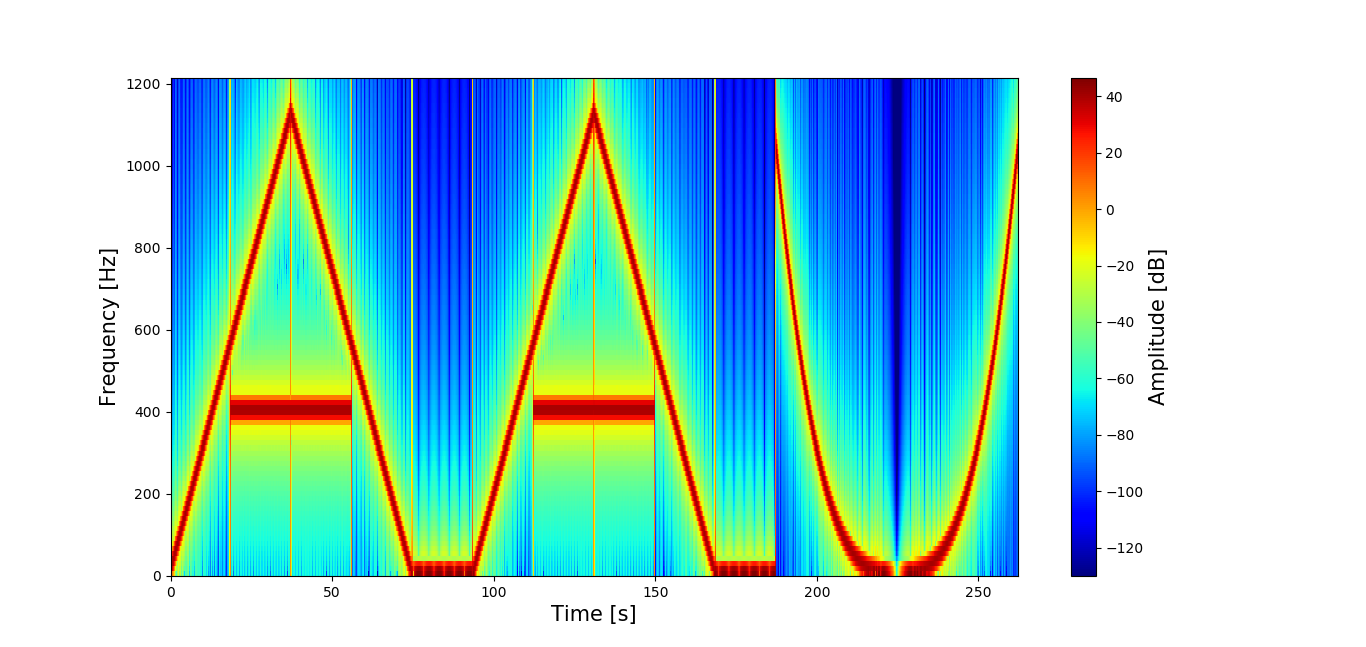
\includegraphics[width=1.4\textwidth]{figures/aaulogo.png}
\end{figure}

  %\vfill
  \begin{center}
  Aalborg University\\
  Department of Mathematical Sciences
  \end{center}
\end{titlepage}
\clearpage

\cleardoublepage
\pdfbookmark[0]{Indholdsfortegnelse}{label:contents}
\pagestyle{fancy} %enable headers and footers again
\tableofcontents

%\listoftodos	

\cleardoublepage
%mainmatter
\pagenumbering{arabic} %use arabic page numbering in the mainmatter
\chapter{Problem analysis} \label{ch1}
In this chapter an introduction will lead to a discussion of problems encountered by a musician when music is to be transcribed. The importance of these problems is analysed and the need for a solution assessed whereafter existing and possible solutions with roots in mathematics will be presented. The chapter will conclude with a \textit{problem statement} which will form the basis for the rest of the project.
\section{Introduction}
Some musicians are capable of playing without reading music written on a sheet of music, and they invent new music through a creative process where they play by ear and do not have the need to write down their compositions. Creative thinking and processes are however interruptable and this can be problematic when the need for transcribing a composition - so as to remember or convey it to others - to a sheet of music arises. This may ruin the creative proces by exactly interrupting it because one needs to concentrate on the transcription.\\\\
To ease the creative process of a musician it is imaginable that some kind of automatic real time transcription of musical compositions can be developed which will eliminate the problem of having to interrupt the aforementioned process.
\section{Problem analysis}
Although the first system of musical notation is the Sumerian system created 3,500 years ago music has existed for much longer. \cite{origins} This means that people have been playing music without any form of written music until then. Even with the creation of standardised musical notation musicianship on high level is possible without any form of education and/or skills in reading and writing music. As such there continue to exist musicians without aforementioned skills.\\\\
Inability to read or write music poses no problem in itself, as it doesn't necessarily hinder musical creativity. Problems however arise when the need to convey or remember musical compositions presents itself. Just as standardised languages make everyday communication and tasks easier a standardised musical notation is needed to convey compositions to others without anyone having to remember the compositions in their entirety. Standard musical notation has been created but has to be learned and research suggests that the ability to read and write music varies considerably from person to person and might even be affected by dyslexia. \cite{dyslexia} In short people are genetically diverse when it comes to learning to read music.\\\\
If musical transcription in the middle of a creative process potentially interrupts said process the effect would be increasingly strengthened by the inability to quickly perform transcriptions which in the worst case scenario would require another person to do the transcription. These consequences of the inability to read/write in musical notation may hinder the distribution of otherwise ingenious musical creations.
\subsection{Existing and possible solutions}
There has been undertaken plenty of research regarding automatic transcription of music and the material is to find in both books \cite{sol1} and articles \cite{sol2}. There also exists downloadable software which helps transcription by hand \cite{transcribe!}. The extensive research done stems from the applications extending to other areas than just transcribing music for musicians - making computers participate with human performances is another imaginable application. Although the research is extensive "[$\hdots$]the performance of transcription systems is still significantly below that of a human expert[$\hdots$]" \cite{future} and so there is room for improvement.\\\\
This project will focus on creating a solution with the use of the mathematical tools of harmonic analysis with the Fourier Transform and of digital filtering to exstract signal information from a digitalized analog signal. The focus will furthermore be on the limitations for this project and the methods used and how these might be overcome. The viability of an algorithm based on the mathematical tools will be tested in a lab to further illustrate the possibilities and limitations of said algorithm. \todo{Her skal måske uddybes, når vi ved mere om vores løsning og metode}
\subsection{Problem statement}
The above analysis is summarized.\\
When musicians compose new music they firstly play but it stunts their creativity when they need to stop to transcribe the music. There is furthermore not necessarily any correlation between musical talent and the ability to transcribe music. This makes it advantageous for many musicians to use a program which automatically transcribes music to a sheet of music. This leads to the following problem statement:
\begin{itemize}
\item[] \textit{How can an algorithm through the use of mathematical tools be designed to automatically transcribe music to a spectrogram?}
\end{itemize}
\section{Limitations}
This project will be limited to focusing on the learning process in designing an algorithm capable of recognizing sound frequencies and translating them to a spectrogram. The spectrogram will furthermore not be a musical score, as this requires complicated algorithms for the recognition of different notes. Instead the spectrogram will show the continuum of frequencies along one axis.\\\\
The music used for testing the algorithm will be simple melodies comtaining one note at a time (no chords) from one instrument at a time. This will allow insight into the methods used without complicating the recognition of notes by blending together different instruments and different sound frequencies.\\\\
The music transcription will be done in non-real time - the designed algorithm will be used on a prerecorded piece of music. This makes it possible to run the algorithm without having to play the piece of music every time and furthermore makes it possible to neglect computational power and/or efficiency.\\\\
As such the end product of this project will ideally be limited to being an algorithm based on mathematical tools which is capable of transcribing a prerecorded piece of simple music to a spectregram. 
%\input{sections/mainmatter/chapter_1/_____.tex}

\chapter{Overskrift} \label{ch2}

\chapter{Musikteori}
I dette kapitel introduceres grundlæggende musikteori, der anvendes i projektet.
\\ \\
I nodesystemet er en node en symbolsk repræsentation af en bestemt tone, som er tilknyttet en specifik frekvens (angivet i hertz, Hz). Hver node indeholder således information om tonens højde og desuden også om dens varighed. Et nodeark er således en symbolsk repræsentation af et diagram over tid og frekvens, hvilket også kaldes et spektrogram.
\\ \\
Til at notere noder benytter man et nodesystem, der består af fem vandrette linjer, hvor noderne er placeret. Grundlæggende findes der 12 forskellige toner Noderne i nodesystemet består først og fremmest af stamtoner, som navngives med bogstaverne A-G afhængigt af deres vertikale placering. Efter G starter navngivningen forfra med det næste A, der ligger en oktav over det forrige. Mellem flere af stamtonerne ligger andre toner, som sammen med stamtonerne udgør de 12 grundtoner, som typisk anvendes i musik. Afstanden mellem alle grundtonerne er en halv tone.

Eksempler på nodernes placeringer fremgår af figur \ref{Cdur}, der er en såkaldt C-dur angivet i G-nøglen. At det er en C-dur betyder, at den starter ved C, går op til G og videre over A, B og til slut C, der ligger en oktav over C. At noderne er angivet i G-nøglen ses ved symbolet i starten af nodesystemet. Der findes mange forskellige nøgler i musik, og G-nøglen angiver, at den nederste tone på figur \ref{Cdur} er det såkaldte nøglehuls-C (der på gamle klaverer ligger ud for nøglehullet), og at A'et mellem den anden- og tredje nederste linje er kammertonen. Kammertonen vælges som definition normalt til at være 440 Hz, men kan dog svinge med $pm 3 Hz$ afhængigt af den enkelte musiker eller orkester, der spiller musikken. Samtlige andre toner i 

\begin{figure}[H]
    \centering
    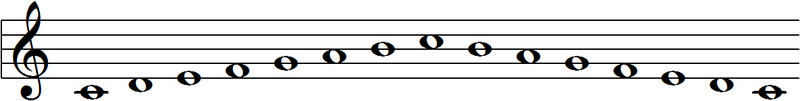
\includegraphics[width = 0.6\textwidth]{figures/C_dur.PNG}
    \caption{C-dur.}
    \label{Cdur}
\end{figure}

I dette projekt betragtes nodesystemet gennem G-nøglen





\chapter{Frekvensanalyse}
I dette kapitel foretages der frekvensanalyse af det samplede signal $s[n]$. Dette gøres for at undersøge signalets frekvensmæssige indhold og fortsætte det videre arbejde med modifikation af signalets indhold.

\section{Dokumentation af algoritmer}
Frekvensanalysen gøres mulig med den diskrete Fouriertransformation (DFT), som beregnes ved hjælp af en \textit{fast Fourier transform}-algoritme (FFT) baseret på Cooley-Tukey algoritmen. Algoritmen er implementeret i Python og udnytter DFT-summens symmetri til at lave en rekursiv opdeling af summen, således den beregningsmæssige kompleksitet nedbringes fra $O(N^2)$ (naiv implementering af DFT) til $O(N\log N)$ for store $N$, hvor $N$ er datalængden. Herunder ses implementeringen af DFT og FFT i et Pythonscript.
\begin{lstlisting}
def DFT(x,c):
    X = np.zeros(c,dtype=complex)
    for k in range(len(x)):
        a = 0+0*1j
        for n in range(c):
            a += x[n]*np.exp(-2*np.pi*1j*k*n/float(c))
            X[k] = a
    return X

def is_power2(num): # Checks if a number is a power of 2
	return num != 0 and ((num & (num - 1)) == 0)

def FFT(x):
    N_new = len(x)
    if is_power2(N_new) == False:
        raise ValueError("N skal vaere en potens af 2.")
    elif N_new == 2:
        return DFT(x,N_new) # Returnerer DFT naar data ikke kan deles mere op
    else:
        X_even = FFT(x[::2]) # Deler rekursivt input op - lige dele
        X_odd = FFT(x[1::2]) # Deler rekursivt input op - ulige dele
        factor = np.exp(-2j * np.pi * np.arange(N_new) / N_new) # Twiddlefaktor
        return np.concatenate([X_even + factor[:int(N_new / 2)] * X_odd,
                               X_even + factor[int(N_new / 2):] * X_odd])
\end{lstlisting}

\section{Tids- og frekvensplot}
I dette afsnit undersøges signalets frekvensspektrum og hvordan dette afhænger af antallet af samples $N$ og samplingsfrekvensen $f_s$. Det vides, at opløsningen i tid afhænger af $f_s$ og at opløsningen i frekvens afhænger af $f_s$ og $N$, således
\begin{align} \label{eq:tidsoploesning}
T = \frac{1}{f_s}\phantom{m}\text{og}\phantom{m} bin=\frac{f_s}{N},
\end{align}

hvor $T$ er samplingsperioden og $bin$ er intervallet mellem to diskrete frekvenser i frekvensdomænet. Dette afsnit undersøger disse relationer.\\
På figur \ref{fig:1} ses signalet i tids- og frekvensdomænet samplet med $f_s=1$ Hz og med $N=2^8, 2^{12}, 2^{18}$ samples.

\begin{figure}[H]
\begin{minipage}{0.49\textwidth}
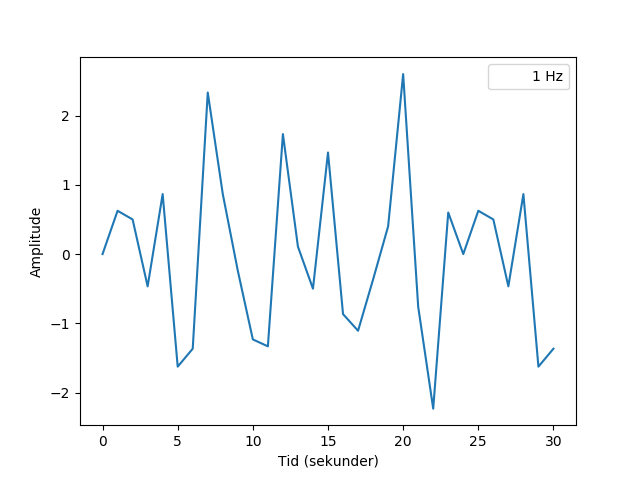
\includegraphics[width=\textwidth]{figures/signal_1hz.png}
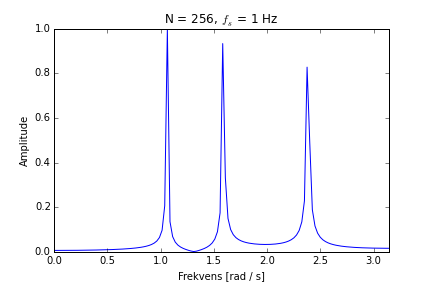
\includegraphics[width=\textwidth]{figures/frekvensanalyse/freq_1hz_N256}
\end{minipage}
\begin{minipage}{0.49\textwidth}
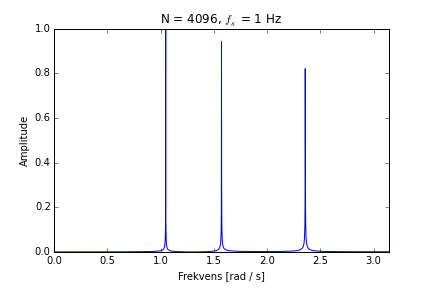
\includegraphics[width=\textwidth]{figures/frekvensanalyse/freq_1hz_N4096.png}
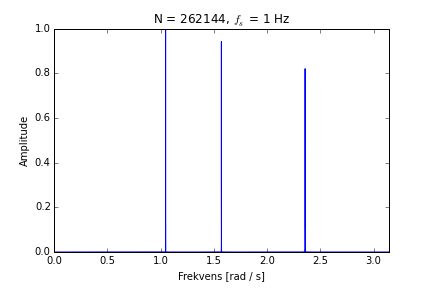
\includegraphics[width=\textwidth]{figures/frekvensanalyse/freq_1hz_N262144.png}
\end{minipage}
\caption{Plot af signal samplet ved $f_s=1$ Hz i tidsdomænet og plot af de tilhørende frekvensdomæner for antal af samples $N = 2^8, 2^{12}, 2^{18}$.}
\label{fig:1}
\end{figure}

På figur \ref{fig:2} ses signalet ligeledes i tids- og frekvensdomænet samplet med $f_s=32$ Hz og med $N=2^8, 2^{12}, 2^{18}$ samples.

\begin{figure}[H]
\begin{minipage}{0.49\textwidth}
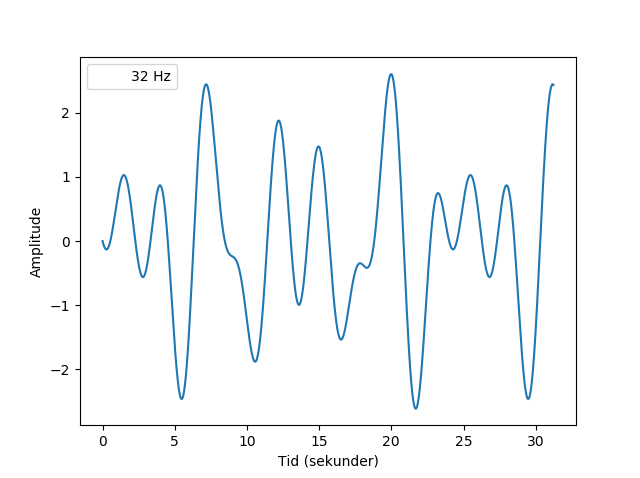
\includegraphics[width=\textwidth]{figures/signal_32hz.png}
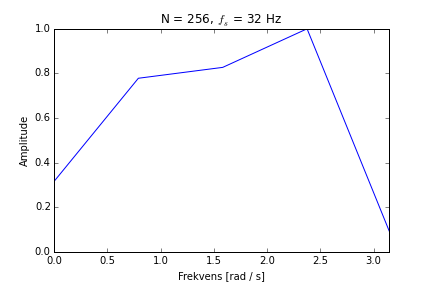
\includegraphics[width=\textwidth]{figures/frekvensanalyse/freq_32hz_N256}
\end{minipage}
\begin{minipage}{0.49\textwidth}
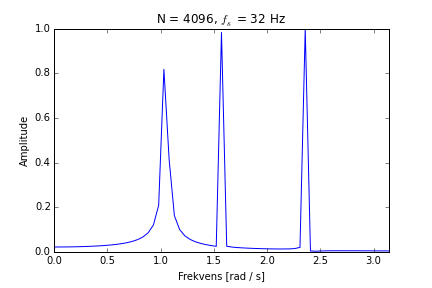
\includegraphics[width=\textwidth]{figures/frekvensanalyse/freq_32hz_N4096.png}
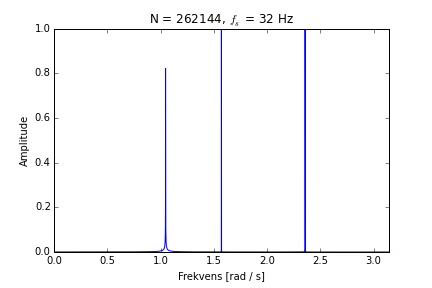
\includegraphics[width=\textwidth]{figures/frekvensanalyse/freq_32hz_N262144.png}
\end{minipage}
\caption{Plot af signal samplet ved $f_s=32$ Hz i tidsdomænet og plot af udsnit af de tilhørende frekvensdomæner for antal af samples $N=2^8, 2^{12}, 2^{18}$.}
\label{fig:2}
\end{figure}

\section{Diskussion}
Det ses tydeligt på tidsdomænerne i figur \ref{fig:1} og figur \ref{fig:2}, at opløsningen af signalet i tid afhænger af $f_s$ og bliver bedre som $f_s$ stiger. Dette stemmer overens med \eqref{eq:tidsoploesning}.
\\ \\
Det ses ligeledes tydeligt, at opløsningen i frekvensdomænet afhænger af $N$ og bliver bedre som $N$ stiger. Det er ydermere bemærkelsesværdigt, at øgning af $f_s$ giver ringere opløsning i frekvensdomænet som set i andet plot i figur \ref{fig:2}. Disse observationer stemmer ligeledes overens med \eqref{eq:tidsoploesning}.
\\ \\
Det ses i figur \ref{fig:1} og \ref{fig:2}, at amplituderne for de tre frekvenser, som signalet indeholder, ikke er lige store, selvom signalet tydeligvis er konstrueret således. Det ses også på figur \ref{fig:1} og figur \ref{fig:2}, at amplituderne varierer som $f_s$ varierer, men ikke som $N$ varierer. Dette skyldes spektral lækage, og er ikke et problem for rekonstruktion af signalet, da energien blot er distribueret rundt om den frekvens, som den bør forefindes ved, således amplituden bliver 1.

%\section{Delkonklusion}
%Frekvensanalysen af signalet afslørede tydeligt de tre frekvenser, som optræder i signalet, og det blev vist, hvordan opløsningen af signalet i tid og frekvens afhænger af $f_s$ og $N$ - bedre opløsning i tid betyder generelt ringere opløsning i frekvens og omvendt. At lade $N$ være arbitrært stor er ikke en mulighed, da den beregningsmæssige kompleksitet afhænger af $N$ og der ikke haves uendelig regnekraft. På baggrund af disse overvejelser skal der træffes en beslutning om fastlæggelsen af $f_s$ og $N$.
\chapter{$\mathcal{L}^p$ and $\ell^p$ spaces} \label{ch4}

This chapter is inspired by \cite{FAA}, \cite{FSP} and \cite{FTFA}.
\\ \\
This project deals with functions in the so-called $\mathcal{L}^p$ and $\ell^p$ spaces. These spaces are introduced in the following and used later to ensure that the Fourier series and transforms used in the project actually converge. The following definitions are inspired by \cite{page 31, FSP}.

\begin{definition}{$\mathcal{L}^p(\mathbb{R})$}
\\
Let $D \subset \mathbb{R}^n$ be a subset. $\mathcal{L}^2(D)$ is the set of all functions on $D$ whose squares are absolutely Lebesgue-integrable over $D$:
\begin{align*}
\mathcal{L}^2(D) = \left\{ f: \int_D |f(x)|^2 dx < \infty \right\}
\end{align*}

$\mathcal{L}^2(D)$ is the normed vector space of square-integrable complex-valued functions. The inner product is:
\begin{align*}
\langle x,y \rangle =  \int_D x(t) \overline{y(t)} dt
\end{align*}

Where $\overline{y(t)}$ is the complex conjugate of $y(t)$. The norm is:
\begin{align*}
\|x\| = \left( \int_D |x(t)|^2 dt \right)^{1/2}
\end{align*}

This definition can be expanded for any $p \in [1,\infty)$ and all of $\mathbb{R}$ such that the normed vector space $\mathcal{L}^p(\mathbb{R})$ is the subspace of $\mathbb{C}^\mathbb{R}$ consisting of vectors with finite $\mathcal{L}^p$ norm:
\begin{align*}
\|x\|_p = \left( \int_{-\infty}^\infty |x(t)|^p dt \right)^{1/p}
\end{align*}
\end{definition}

As stated in \cite{page 74, FAA}, this space is simply the space of all functions $f$ such that the region between the graph of $|f|^2$ and the $x$-axis has finite area. The Lebesgue integral is therefore just another way of calculating the area between the graph of the function and the $x$-axis. The Lebesgue integral will not be elaborated further in this project as it is beyond its focus.
\\ \\
A similar definition is given for $\ell^p$ which deals with sequences:
\begin{definition}{$\ell^p(\mathbb{Z})$}
\\
$\ell^2(\mathbb{Z})$ is the space of square-summable sequences, and the inner product is defined as:
\begin{align*}
\langle x,y \rangle = \sum_{n\in\mathbb{Z}} x[n] \overline{y[n]}
\end{align*}

And the norm is defined as:
\begin{align*}
\|x\| = \left( \sum_{n\in\mathbb{Z}} |x[n]|^2 \right)^{1/2}
\end{align*}

For any $p \in [1,\infty)$, the normed vector space $\ell^p(\mathbb{Z})$ is the subspace of $\mathbb{C}^N$ consisting of vectors with finite $\ell^p$ norm:
\begin{align*}
\|x\|_p = \left( \sum_{n\in\mathbb{Z}} |x[n]|^p \right)^{1/p}
\end{align*}

Furthermore, the $\ell^\infty$ norm is defined as:
\begin{align*}
\|x\|_\infty = \sup_{n\in\mathbb{Z}}|x[n]|
\end{align*}
\end{definition}


Noter fra vejledermødet 28-02-2017:
\begin{align*}
\|f\|_{L^p} = \left( \int_{-\infty}^\infty |f(x)|^p dx \right)^{1/p} \\
\langle f,g \rangle = \int_{-\infty}^\infty f(x) \overline{g(x)} dx
\end{align*}
(ligesom angivet ovenfor). Hvis $f \in L^1$ eller $L^2$ og $g \in L^1$ (mindst én i $L^1$), så gælder der:
\begin{align*}
F(f*g) = \hat{f} \cdot \hat{g}
\end{align*}

Altså er foldning i tidsdomænet det samme som at gange i frekvensdomænet.

\begin{align*}
L^p(\mathbb{R}) =
\left\{\begin{matrix}
f : \mathbb{R} \to \mathbb{C}: \int_{-\infty}^\infty |f(x)|^p dx < \infty \\
Measureable (integrationsteori)
\end{matrix}\right.
\end{align*}

$$

%The following should be rewritten as it is almost copied directly from the book.
%\\ \\
%From Folland, p. 81-82:
%One can replace the element $dx$ of linear measure on $[a,b]$ by a weighted element of measure, $w(x) dx$. To be precise, suppose $w$ is a continuous function on $[a,b]$ such that $w(x) > 0$ for all $x \in [a,b]$; we call such a $w$ a weight function on $[a,b]$. We can then define the weighted $L^2$ space $L^2_w(a,b)$ to be the set of all (Lebesgue measurable) functions on $[a,b]$ such that
%\begin{align*}
%\int_a^b |f(x)|^2 w(x) dx < \infty,
%\end{align*}
%
%and we define an inner product and norm on $L_w^2(a,b)$ by
%\begin{align*}
%\langle f,g \rangle = \int_a^b f(x) \overline{g(x)} w(x) dx, \quad \|f\|_w = \left( \int_a^b |f(x)|^2 w(x) dx \right)^{1/2}
%\end{align*}
%
%We define $L_2(D)$ to be the set of all functions $f$ such that:
%\begin{align*}
%\int_D |f(\textbf{x})|^2 d\textbf{x} < \infty
%\end{align*}
%
%and we define the inner product and norm on $L^2(D)$ by
%\begin{align*}
%\langle f,g \rangle = \int_D f(\textbf{x}) \overline{g(\textbf{x})} d \textbf{x}, \quad \|f\| = \left( \int_D |f(\textbf{x})|^2 d \textbf{x} \right)^{1/2}.
%\end{align*}
%
%Another example of a Hilbert space is the space $l^2$ of square-summable sequences. That is, the elements of $l^2$ are sequences $\{c_n\}_1^\infty$ of complex numbers such that $\sum_1^\infty |c_n|^2 < \infty$, and the inner product and norm are defined by
%\begin{align*}
%\left\langle \{c_n\},\{d_n\} \right\rangle = \sum_1^\infty c_n \overline{d}_n, \quad \left\| \{c_n\} \right\| = \left( \sum_1^\infty  |c_n|^2 \right)^{1/2}
%\end{align*}
%\\ \\
%From M. Vetterli, page 35:
%$\mathcal{L}^p(\mathbb{R})$ spaces Like for sequences, we can define other norms on $\mathbb{C}^\mathbb{R}$ as well. Again, because the space is infinite-dimensional, the choice of the norm and the requirement that it be finite restricts $\mathbb{C}^\mathbb{R}$ to a smaller set. For example, for $p \in [1,\infty)$, the $\mathcal{L}^p$ norm is
%\begin{align*}
%\|x\|_p = \left( \int_{-\infty}^{\infty} |x(t)|^p dt \right)^{1/p}
%\end{align*}
%
%The extension to $p = \infty$ leads to the $\mathcal{L}^\infty$ norm as
%\begin{align*}
%\|x\|_\infty = ess \sup_{t\in\mathbb{R}} |x(t)|.
%\end{align*}



\printbibliography[heading=bibintoc]
\label{bib:mybiblio}
\appendix
\chapter{Bilag}
\section{Udledning af den ideelle impulsrespons} \label{app1}
For at udlede den ideelle impulsrespons defineres først den ideelle frekvensrespons som følger på baggrund af filterets specifikationer defineret i sektion \ref{ch4_specs}.
\begin{align*}
 H_d(\text{e}^{j\omega})= \begin{cases}
  \text{e}^{-j\omega\frac{M}{2}}, \ \ \ & |\omega| \leq\omega_{c_1} \\
 0, \ \ \ & \omega_{c_1} \leq |\omega| \leq \omega_{c_2} \\
  \text{e}^{-j\omega\frac{M}{2}}, \ \ \ & \omega_{c_2} \leq |\omega| 
\end{cases}
\end{align*}
  
Herudfra bestemmes den ideelle impulsrespons ved hjælp af den inverse Fourier-transformation:
\begin{align*}
h_d[n] &= \frac{1}{2\pi} \left(  \int_{-\pi}^{-\omega_{c_2}} \text{e}^{-j\omega \frac{M}{2}} \cdot \text{e}^{j \omega n} d\omega + \int_{-\omega_{c_1}}^{\omega_{c_1}} \text{e}^{-j\omega \frac{M}{2}} \cdot \text{e}^{j \omega n} d\omega +\int_{\omega_{c_2}}^{\pi} \text{e}^{-j\omega \frac{M}{2}} \cdot \text{e}^{j \omega n} d\omega	\right) \\
&= \frac{1}{2\pi} \left(  \int_{-\pi}^{-\omega_{c_2}} \text{e}^{j\omega \left(n- \frac{M}{2} \right) } d\omega + \int_{-\omega_{c_1}}^{\omega_{c_1}} \text{e}^{j\omega \left(n- \frac{M}{2} \right) }  d\omega + \int_{\omega_{c_2}}^{\pi} \text{e}^{j\omega \left( n-\frac{M}{2} \right) } d\omega	\right).
\end{align*}

Her udnyttes det nu, at der gælder:
\begin{align*}
\int_{-\pi}^{\pi} \text{e}^{j\omega \left(n- \frac{M}{2} \right) }  d\omega =& \int_{-\pi}^{\pi} \cos\left( \omega \left(n-\frac{M}{2}\right)\right)+j \sin \left( \omega \left(n-\frac{M}{2}\right) \right) d\omega \\
=& \left[ \sin\left(\omega \left(n-\frac{M}{2}\right)\right) \right]_{-\pi}^{\pi} \cdot \frac{1}{n- \frac{M}{2}}.
\end{align*}

Således fås:
\begin{align*}
h_d[n]= \frac{1}{\pi \left(n-\frac{M}{2}\right)} \left(\sin\left(\omega_{c_2} \left(n-\frac{M}{2}\right)\right) - \sin\left(\omega_{c_1} \left(n-\frac{M}{2}\right)\right) - \sin\left( \pi\left( n + \frac{M}{2} \right) \right) \right).
\end{align*}

Da sidste led må være $0$ defineres den ideelle impulsrespons som følger:
\begin{align*}
h_d[n]= \frac{1}{\pi \left(n-\frac{M}{2}\right)} \left(\sin\left(\omega_{c_2} \left(n-\frac{M}{2}\right)\right) - \sin\left(\omega_{c_1} \left(n-\frac{M}{2}\right)\right)\right)
\end{align*}

Dette gælder dog kun for $n \neq 0$, og dermed defineres $h_d[0]$ seperat. Hertil anvendes l'Hôspitals regel, som siger, at $\lim \frac{f(x)}{g(x)}=\lim \frac{f'(x)}{g'(x)}$.
\begin{align*}
h_d[0]=& \frac{1}{\pi} \left( \cos\left( \omega_{c_1} \left(n-\frac{M}{2}\right) \right)\omega_{c_1} - \cos\left( \omega_{c_2} \left(n-\frac{M}{2}\right) \right)\omega_{c_2} +  \cos\left(\pi \left( n- \frac{M}{2}\right) \right) \pi \right) \\
=& \frac{1}{\pi}\left( \omega_{c_1} - \omega_{c_2} + \pi \right) \\
=& 1 - \frac{\omega_{c_2}-\omega_{c_1}}{\pi}
\end{align*}

\section{Amplituderespons for filteret} \label{app2}

\begin{figure}[H]
\begin{minipage}{0.49\textwidth}
\centering
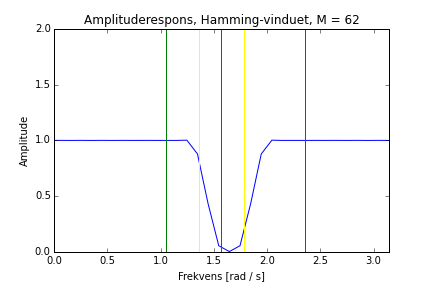
\includegraphics[width=\textwidth]{figures/Filter/Filter_Hamming_62.png}
\end{minipage}
\begin{minipage}{0.49\textwidth}
\centering
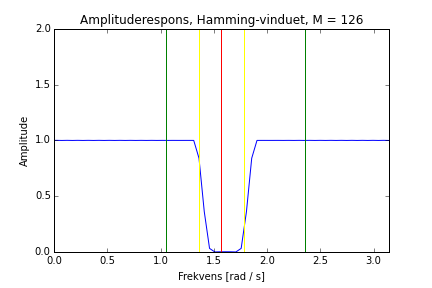
\includegraphics[width=\textwidth]{figures/Filter/Filter_Hamming_126.png}
\end{minipage}
\caption{Amplituderesponser for filteret af orden $M = 62$ og $M=126$ ved anvendelse af Hamming-vinduet.}
\label{fig:amplituderespons_Hamming}
\end{figure}
\chapter{Bilag}\label{app2}
\section{Amplituderespons for Hammingvindue}
\begin{figure}
\centering
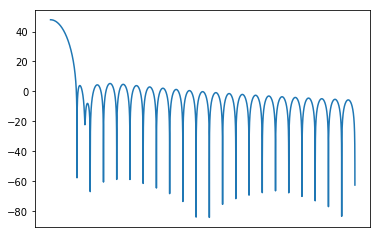
\includegraphics[width=0.7\textwidth]{figures/amplituderespons.png}
\caption{Amplituderespons for Hammingvidue af orden $M=92$.}
\label{fig:amplituderespons}
\end{figure}

\end{document}